\documentclass[journal,12pt,twocolumn]{IEEEtran}
\usepackage{setspace}
\usepackage{gensymb}
\usepackage{caption}
%\usepackage{multirow}
%\usepackage{multicolumn}
%\usepackage{subcaption}
%\doublespacing
\singlespacing
\usepackage{csvsimple}
\usepackage{amsmath}
\usepackage{multicol}
\usepackage{enumerate}
\usepackage{amssymb}
\usepackage{graphicx}
\usepackage{newfloat}
%\usepackage{syntax}
\usepackage{listings}
%\usepackage{iithtlc}
\usepackage{color}
\usepackage{tikz}
\usetikzlibrary{shapes,arrows}



%\usepackage{graphicx}
%\usepackage{amssymb}
%\usepackage{relsize}
%\usepackage[cmex10]{amsmath}
%\usepackage{mathtools}
%\usepackage{amsthm}
%\interdisplaylinepenalty=2500
%\savesymbol{iint}
%\usepackage{txfonts}
%\restoresymbol{TXF}{iint}
%\usepackage{wasysym}
\usepackage{amsthm}
\usepackage{mathrsfs}
\usepackage{txfonts}
\usepackage{stfloats}
\usepackage{cite}
\usepackage{cases}
\usepackage{mathtools}
\usepackage{caption}
\usepackage{enumerate}	
\usepackage{enumitem}
\usepackage{amsmath}
%\usepackage{xtab}
\usepackage{longtable}
\usepackage{multirow}
%\usepackage{algorithm}
%\usepackage{algpseudocode}
\usepackage{enumitem}
\usepackage{mathtools}
\usepackage{hyperref}
%\usepackage[framemethod=tikz]{mdframed}
\usepackage{listings}
    %\usepackage[latin1]{inputenc}                                 %%
    \usepackage{color}                                            %%
    \usepackage{array}                                            %%
    \usepackage{longtable}                                        %%
    \usepackage{calc}                                             %%
    \usepackage{multirow}                                         %%
    \usepackage{hhline}                                           %%
    \usepackage{ifthen}                                           %%
  %optionally (for landscape tables embedded in another document): %%
    \usepackage{lscape}     


\usepackage{url}
\def\UrlBreaks{\do\/\do-}


%\usepackage{stmaryrd}


%\usepackage{wasysym}
%\newcounter{MYtempeqncnt}
\DeclareMathOperator*{\Res}{Res}
%\renewcommand{\baselinestretch}{2}
\renewcommand\thesection{\arabic{section}}
\renewcommand\thesubsection{\thesection.\arabic{subsection}}
\renewcommand\thesubsubsection{\thesubsection.\arabic{subsubsection}}

\renewcommand\thesectiondis{\arabic{section}}
\renewcommand\thesubsectiondis{\thesectiondis.\arabic{subsection}}
\renewcommand\thesubsubsectiondis{\thesubsectiondis.\arabic{subsubsection}}

% correct bad hyphenation here
\hyphenation{op-tical net-works semi-conduc-tor}

%\lstset{
%language=C,
%frame=single, 
%breaklines=true
%}

%\lstset{
	%%basicstyle=\small\ttfamily\bfseries,
	%%numberstyle=\small\ttfamily,
	%language=Octave,
	%backgroundcolor=\color{white},
	%%frame=single,
	%%keywordstyle=\bfseries,
	%%breaklines=true,
	%%showstringspaces=false,
	%%xleftmargin=-10mm,
	%%aboveskip=-1mm,
	%%belowskip=0mm
%}

%\surroundwithmdframed[width=\columnwidth]{lstlisting}
\def\inputGnumericTable{}                                 %%
\lstset{
%language=C,
frame=single, 
breaklines=true,
columns=fullflexible
}
 

\begin{document}
%
\tikzstyle{block} = [rectangle, draw,
    text width=3em, text centered, minimum height=3em]
\tikzstyle{sum} = [draw, circle, node distance=3cm]
\tikzstyle{input} = [coordinate]
\tikzstyle{output} = [coordinate]
\tikzstyle{pinstyle} = [pin edge={to-,thin,black}]

\theoremstyle{definition}
\newtheorem{theorem}{Theorem}[section]
\newtheorem{problem}{Problem}
\newtheorem{proposition}{Proposition}[section]
\newtheorem{lemma}{Lemma}[section]
\newtheorem{corollary}[theorem]{Corollary}
\newtheorem{example}{Example}[section]
\newtheorem{definition}{Definition}[section]
%\newtheorem{algorithm}{Algorithm}[section]
%\newtheorem{cor}{Corollary}
\newcommand{\BEQA}{\begin{eqnarray}}
\newcommand{\EEQA}{\end{eqnarray}}
\newcommand{\define}{\stackrel{\triangle}{=}}
\bibliographystyle{IEEEtran}
%\bibliographystyle{ieeetr}
\providecommand{\nCr}[2]{\,^{#1}C_{#2}} % nCr
\providecommand{\nPr}[2]{\,^{#1}P_{#2}} % nPr
\providecommand{\mbf}{\mathbf}
\providecommand{\pr}[1]{\ensuremath{\Pr\left(#1\right)}}
\providecommand{\qfunc}[1]{\ensuremath{Q\left(#1\right)}}
\providecommand{\sbrak}[1]{\ensuremath{{}\left[#1\right]}}
\providecommand{\lsbrak}[1]{\ensuremath{{}\left[#1\right.}}
\providecommand{\rsbrak}[1]{\ensuremath{{}\left.#1\right]}}
\providecommand{\brak}[1]{\ensuremath{\left(#1\right)}}
\providecommand{\lbrak}[1]{\ensuremath{\left(#1\right.}}
\providecommand{\rbrak}[1]{\ensuremath{\left.#1\right)}}
\providecommand{\cbrak}[1]{\ensuremath{\left\{#1\right\}}}
\providecommand{\lcbrak}[1]{\ensuremath{\left\{#1\right.}}
\providecommand{\rcbrak}[1]{\ensuremath{\left.#1\right\}}}
\theoremstyle{remark}
\newtheorem{rem}{Remark}
\newcommand{\sgn}{\mathop{\mathrm{sgn}}}
\providecommand{\abs}[1]{\left\vert#1\right\vert}
\providecommand{\res}[1]{\Res\displaylimits_{#1}} 
\providecommand{\norm}[1]{\left\Vert#1\right\Vert}
\providecommand{\mtx}[1]{\mathbf{#1}}
\providecommand{\mean}[1]{E\left[ #1 \right]}
\providecommand{\fourier}{\overset{\mathcal{F}}{ \rightleftharpoons}}
%\providecommand{\hilbert}{\overset{\mathcal{H}}{ \rightleftharpoons}}
\providecommand{\system}{\overset{\mathcal{H}}{ \longleftrightarrow}}
	%\newcommand{\solution}[2]{\textbf{Solution:}{#1}}
\newcommand{\solution}{\noindent \textbf{Solution: }}
\newcommand{\myvec}[1]{\ensuremath{\begin{pmatrix}#1\end{pmatrix}}}
\providecommand{\dec}[2]{\ensuremath{\overset{#1}{\underset{#2}{\gtrless}}}}
\DeclarePairedDelimiter{\ceil}{\lceil}{\rceil}
%\numberwithin{equation}{section}
%\numberwithin{problem}{subsection}
%\numberwithin{definition}{subsection}
\makeatletter
\@addtoreset{figure}{section}
\makeatother
\let\StandardTheFigure\thefigure
%\renewcommand{\thefigure}{\theproblem.\arabic{figure}}
\renewcommand{\thefigure}{\thesection}
%\numberwithin{figure}{subsection}
%\numberwithin{equation}{subsection}
%\numberwithin{equation}{section}
%\numberwithin{equation}{problem}
%\numberwithin{problem}{subsection}
\numberwithin{problem}{section}
%%\numberwithin{definition}{subsection}
%\makeatletter
%\@addtoreset{figure}{problem}
%\makeatother
\makeatletter
\@addtoreset{table}{section}
\makeatother
\let\StandardTheFigure\thefigure
\let\StandardTheTable\thetable
\let\vec\mathbf
\numberwithin{equation}{section}
\vspace{3cm}
% \title{%Convex Optimization in Python
% 	\logo{
% 	Random Numbers
% 	}
% }
%\title{
%	\logo{Matrix Analysis through Octave}{\begin{center}\includegraphics[scale=.24]{tlc}\end{center}}{}{HAMDSP}
%}
% paper title
% can use linebreaks \\ within to get better formatting as desired
%\title{Matrix Analysis through Octave}
%
%
% author names and IEEE memberships
% note positions of commas and nonbreaking spaces ( ~ ) LaTeX will not break
% a structure at a ~ so this keeps an author's name from being broken across
% two lines.
% use \thanks{} to gain access to the first footnote area
% a separate \thanks must be used for each paragraph as LaTeX2e's \thanks
% was not built to handle multiple paragraphs
%
\author{ Pradeep Mundlik% <-this % stops a space
% <-this % stops a space
%\thanks{J. Doe and J. Doe are with Anonymous University.}% <-this % stops a space
%\thanks{Manuscript received April 19, 2005; revised January 11, 2007.}}
}
% note the % following the last \IEEEmembership and also \thanks - 
% these prevent an unwanted space from occurring between the last author name
% and the end of the author line. i.e., if you had this:
% 
% \author{....lastname \thanks{...} \thanks{...} }
%                     ^------------^------------^----Do not want these spaces!
%
% a space would be appended to the last name and could cause every name on that
% line to be shifted left slightly. This is one of those "LaTeX things". For
% instance, "\textbf{A} \textbf{B}" will typeset as "A B" not "AB". To get
% "AB" then you have to do: "\textbf{A}\textbf{B}"
% \thanks is no different in this regard, so shield the last } of each \thanks
% that ends a line with a % and do not let a space in before the next \thanks.
% Spaces after \IEEEmembership other than the last one are OK (and needed) as
% you are supposed to have spaces between the names. For what it is worth,
% this is a minor point as most people would not even notice if the said evil
% space somehow managed to creep in.
% The paper headers
%\markboth{Journal of \LaTeX\ Class Files,~Vol.~6, No.~1, January~2007}%
%{Shell \MakeLowercase{\textit{et al.}}: Bare Demo of IEEEtran.cls for Journals}
% The only time the second header will appear is for the odd numbered pages
% after the title page when using the twoside option.
% 
% *** Note that you probably will NOT want to include the author's ***
% *** name in the headers of peer review papers.                   ***
% You can use \ifCLASSOPTIONpeerreview for conditional compilation here if
% you desire.
% If you want to put a publisher's ID mark on the page you can do it like
% this:
%\IEEEpubid{0000--0000/00\$00.00~\copyright~2007 IEEE}
% Remember, if you use this you must call \IEEEpubidadjcol in the second
% column for its text to clear the IEEEpubid mark.
% make the title area
\title{Assignment}
\maketitle
\tableofcontents
% \bigskip
\renewcommand{\thefigure}{\theenumi}
\renewcommand{\thetable}{\theenumi}
%%

\section{Uniform Random Numbers}
Let $U$ be a uniform random variable between 0 and 1.
\begin{enumerate}[label=\thesection.\arabic*
,ref=\thesection.\theenumi]
\item Generate $10^6$ samples of $U$ using a C program and save into a file called uni.dat .
\\
\solution Download the following files and execute the  C program.
\begin{lstlisting}
	https://github.com/PradeepMundlik/AI1110/blob/master/Assignment_Soln/codes/1/exrand.c 
\end{lstlisting}
\begin{lstlisting}
	https://github.com/PradeepMundlik/AI1110/blob/master/Assignment_Soln/codes/coeffs.h
\end{lstlisting}

%
\item
Load the uni.dat file into python and plot the empirical CDF of $U$ using the samples in uni.dat. The CDF is defined as
\begin{align}
F_{U}(x) = \pr{U \le x}
\end{align}
\\
\solution  The following code plots Fig. \ref{fig:uni_cdf}
\begin{lstlisting}
	https://github.com/PradeepMundlik/AI1110/blob/master/Assignment_Soln/codes/1/cdf_plot.py
\end{lstlisting}
\begin{figure}[h]
\centering
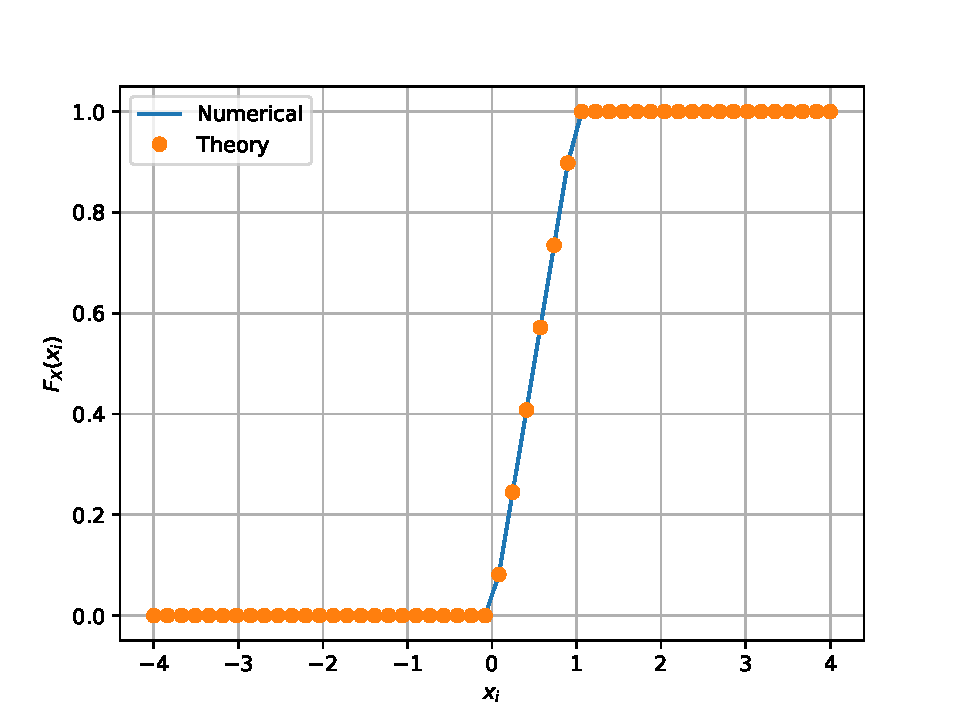
\includegraphics[width=\columnwidth]{figs/1/uni_cdf.pdf}
\caption{The CDF of $U$}
\label{fig:uni_cdf}
\end{figure}

%
\item
Find a  theoretical expression for $F_{U}(x)$. \\
\solution
As U is uniform random variable distribution, (between 0 to 1);
$CDF = F_U(x)$
\begin{align}
	F_U(x) = \int_{0}^{x} P_U(x) \,dx 
\end{align}
As uniform distribution, $P_U(x_i) = t$ (t is constant) \\
So,
\begin{align}
	F_U(x) = \int_{0}^{x} t \,dx 
\end{align}
We know that,
\begin{align}
	&F_U(1) = 1 \\
	\implies &\int_{0}^{1} t \,dx = 1 \\
	\implies &t = 1 \\
	\implies &F_U(x) = \int_{0}^{x} 1 \,dx \\
	\implies &F_U(x) = x
\end{align}

\item
The mean of $U$ is defined as
%
\begin{equation}
E\sbrak{U} = \frac{1}{N}\sum_{i=1}^{N}U_i
\end{equation}
%
and its variance as
%
\begin{equation}
\text{var}\sbrak{U} = E\sbrak{U- E\sbrak{U}}^2 
\end{equation}

Write a C program to  find the mean and variance of $U$. \\
\solution
Code file can be found here:
\begin{lstlisting}
	https://github.com/PradeepMundlik/AI1110/blob/master/Assignment_Soln/codes/1/q1_4.c
\end{lstlisting}
Mean=0.500007 \\
Variance=0.083301
\item Verify your result theoretically given that
\end{enumerate}
%
\begin{equation}
E\sbrak{U^k} = \int_{-\infty}^{\infty}x^kdF_{U}(x)
\end{equation}
\solution
from question 1.3 \\
\begin{align}
	F_U(x) = x \\
	E\sbrak{U^k} = \int_{-\infty}^{\infty}x^kdx 
\end{align}
for k = 1,
\begin{align}
	E\sbrak{U} &= \int_{-\infty}^{\infty}xdx \\
	 &= \int_{0}^{1}xdx \\
	 &= \frac{1}{2}
\end{align}
for k = 2,
\begin{align}
	E\sbrak{U^2} &= \int_{-\infty}^{\infty}x^2dx \\
	 &= \int_{0}^{1}x^2dx + 0 \\
	 &= \frac{1}{3}
\end{align}
Mean = 0.5 \\
\begin{align}
	var(x) &= E[U^2] - (E\sbrak{U})^2 \\
	 &= \frac{1}{3} - \left(\frac{1}{2}\right)^2 \\
	 &= \frac{1}{3} - \frac{1}{4} \\
	 &= \frac{1}{12} \\
	 var(x) &= 0.083
\end{align}
\section{Central Limit Theorem}
%
\begin{enumerate}[label=\thesection.\arabic*
,ref=\thesection.\theenumi]

%
\item
Generate $10^6$ samples of the random variable
%
\begin{equation}
X = \sum_{i=1}^{12}U_i -6
\end{equation}
%
using a C program, where $U_i, i = 1,2,\dots, 12$ are  a set of independent uniform random variables between 0 and 1
and save in a file called gau.dat \\
\solution 
\begin{lstlisting}
	https://github.com/PradeepMundlik/AI1110/blob/master/Assignment_Soln/codes/2/q2_1.c
\end{lstlisting}
%
\item
Load gau.dat in python and plot the empirical CDF of $X$ using the samples in gau.dat. What properties does a CDF have?
\\
\solution The CDF of $X$ is plotted in Fig. \ref{fig:gauss_cdf} \\
\begin{lstlisting}
	https://github.com/PradeepMundlik/AI1110/blob/master/Assignment_Soln/codes/2/cdf_plot.py
\end{lstlisting}
\begin{figure}[h]
\centering
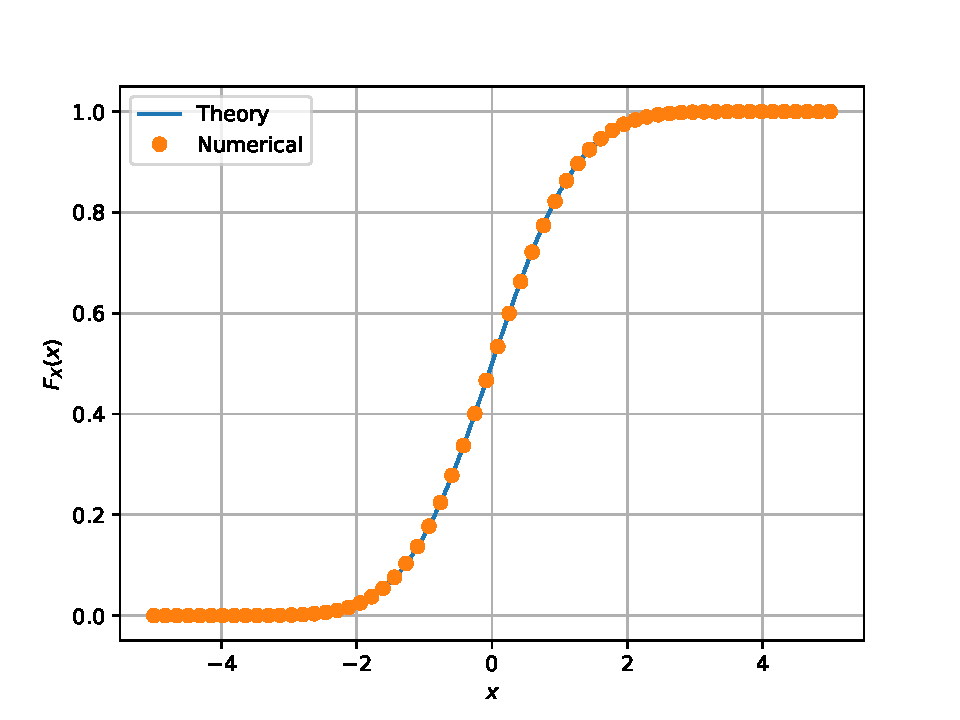
\includegraphics[width=\columnwidth]{figs/2/gau_cdf.pdf}
\caption{The CDF of $X$}
\label{fig:gauss_cdf}
\end{figure}
Properties of CDF:
\begin{itemize}
	\item As x reaches 0 the CDF reaches 0.5 
	\item As x approaches infinity the CDF approaches 1
	\item As x approaches minus infinity the CDF approaches 0 
\end{itemize}
\item
Load gau.dat in python and plot the empirical PDF of $X$ using the samples in gau.dat. The PDF of $X$ is defined as
\begin{align}
p_{X}(x) = \frac{d}{dx}F_{X}(x)
\end{align}
What properties does the PDF have?
\\
\solution The PDF of $X$ is plotted in Fig. \ref{fig:gauss_pdf} using the code below
\begin{lstlisting}
	https://github.com/PradeepMundlik/AI1110/blob/master/Assignment_Soln/codes/2/pdf_plot.py
\end{lstlisting}
Proprties of PDF of X:
\begin{itemize}
	\item Graph is simitrical about x=0
	\item Graph have its peak at x=0
\end{itemize}
\begin{figure}[h]
\centering
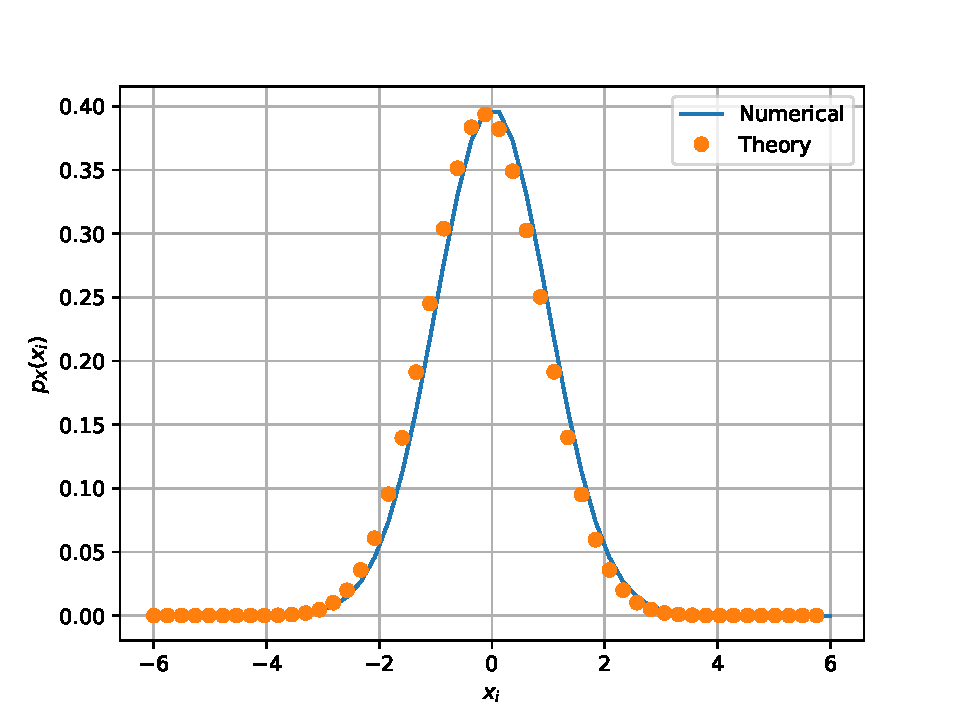
\includegraphics[width=\columnwidth]{figs/2/gauss_pdf.pdf}
\caption{The PDF of $X$}
\label{fig:gauss_pdf}
\end{figure}

\item Find the mean and variance of $X$ by writing a C program. \\
\solution \\
 Mean = 0.000294 \\
 Variance = 0.999560 \\
 c code file can be found at below link:
\begin{lstlisting}
	https://github.com/PradeepMundlik/AI1110/blob/master/Assignment_Soln/codes/2/q2_4.c
\end{lstlisting}
\item Given that 
\begin{align}
p_{X}(x) = \frac{1}{\sqrt{2\pi}}\exp\brak{-\frac{x^2}{2}}, -\infty < x < \infty,
\end{align}
repeat the above exercise theoretically.
\solution
\begin{align}
	&E[x] = \int_{-\infty}^{\infty} xp_X(x) \,dx \\
	&E[x] = \int_{-\infty}^{\infty} x\frac{1}{\sqrt{2\pi}}\exp\brak{-\frac{x^2}{2}} \,dx \\
	&E[x] = \frac{1}{\sqrt{2\pi}}\int_{-\infty}^{\infty} x\exp\brak{-\frac{x^2}{2}} \,dx \\
	&\frac{x^2}{2} = t \\
	&xdx = dt \\
	&E[x] = \frac{1}{\sqrt{2\pi}} \int_{\infty}^{\infty} \exp(-t) \, dt \\
	&E[x] = 0 \\
	&E[x^2] = \int_{-\infty}^{\infty} x^2p_X(x) \,dx \\
	&E[x^2] = \frac{1}{\sqrt{2\pi}}\int_{-\infty}^{\infty} x^2 \exp\brak{-\frac{x^2}{2}}\,dx \\
	&E[x^2] = \frac{1}{\sqrt{2\pi}}\int_{-\infty}^{\infty} x\left(x \exp\brak{-\frac{x^2}{2}}\right)\,dx \\
\end{align}
Integration by parts,
\begin{align}
	 = x I \,dx - \int I \,dx 
\end{align}
Where $I = \int x \exp\brak{-\frac{x^2}{2}}$ \\
\begin{align}
	\frac{x^2}{2} = t \\
	I = \int \exp(-t) \, dt \\
	I = -\exp(-t) \\
	I = -\exp\brak{-\frac{x^2}{2}} \\
\end{align}
from (2.15),
\begin{align}
	 = -x\exp\brak{-\frac{x^2}{2}} - \int -\exp\brak{-\frac{x^2}{2}} \,dx \\
	 = -x\exp\brak{-\frac{x^2}{2}} + \int \exp\brak{-\frac{x^2}{2}} \,dx 
\end{align}
Substituting limits in (2.13),
\begin{align}
	&E[x^2] = \frac{1}{\sqrt{2\pi}} \int_{-\infty}^{\infty} \exp\brak{-\frac{x^2}{2}} \\
	&E[x^2] = \frac{1}{\sqrt{2\pi}} \times \sqrt{2\pi} \\
	&E[x^2] = 1 \\
	&Var(x) = E[x^2] - \left(E[x]\right)^2 \\
	&Var(x) = 1 - 0 \\
	&Var(x) = 1
\end{align}
\end{enumerate}

\section{From Uniform to Other}
\begin{enumerate}[label=\thesection.\arabic*
,ref=\thesection.\theenumi]
%
\item
Generate samples of 
%
\begin{equation}
V = -2\ln\brak{1-U}
\end{equation}
%
and plot its CDF. \\
\solution 
Code for plot can be found at below link:
\begin{lstlisting}
	https://github.com/PradeepMundlik/AI1110/blob/master/Assignment_Soln/codes/3/q3_1.py
\end{lstlisting}
\begin{lstlisting}
	https://github.com/PradeepMundlik/AI1110/blob/master/Assignment_Soln/codes/3/q3_1.dat
\end{lstlisting}
\begin{figure}[h]
	\centering
	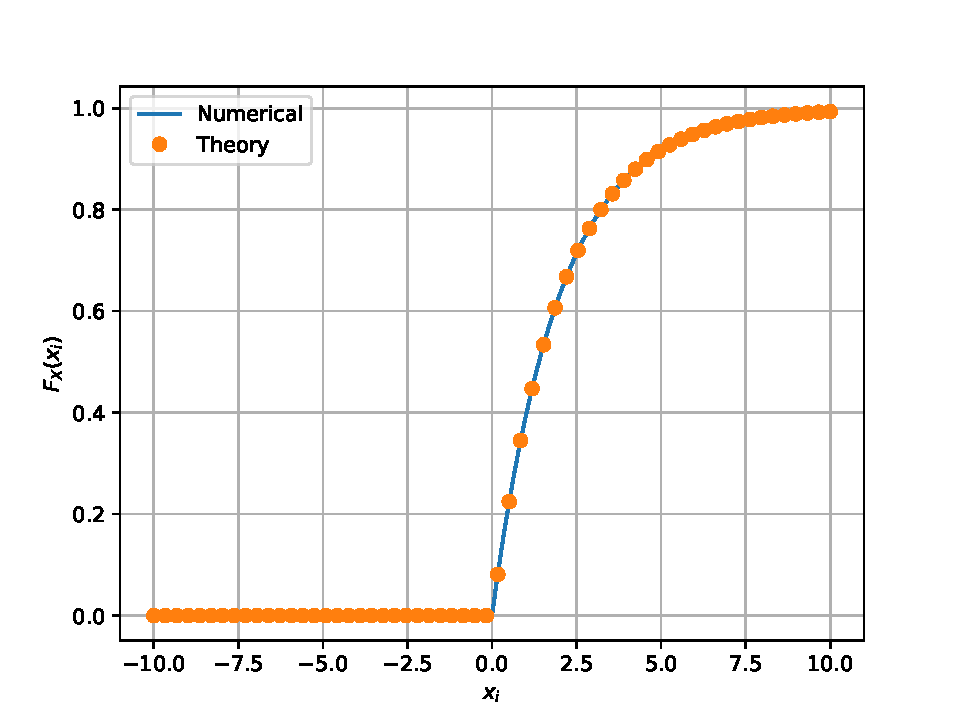
\includegraphics[width=\columnwidth]{figs/3/q3_1.pdf}
	\caption{The CDF of $V$}
	\label{fig:cdf_v}
	\end{figure}
\item Find a theoretical expression for $F_V(x)$. \\
\solution 
\begin{align}
	&F_V(x) = P(V < x) \\
	&F_V(x) = P(-2 \ln(1-U) < x) \\
	&F_V(x) = P\left((1-U) > \exp\brak{-\frac{x}{2}}\right) \\
	&F_V(x) = P\left(U < 1 - \exp\brak{-\frac{x}{2}}\right) \\
	&P(U < x) = x \\
	&P\left(U < 1 - \exp\brak{-\frac{x}{2}}\right) = 1 - \exp\brak{-\frac{x}{2}} \\
	&F_V(x) = 1 - \exp\brak{-\frac{x}{2}}
\end{align}

%
%\item
%Generate the Rayleigh distribution from Uniform. Verify your result through graphical plots.
\end{enumerate}

\section{Triangular Distribution}
\begin{enumerate}[label=\thesection.\arabic*
,ref=\thesection.\theenumi]
%
\item Generate 
	\begin{align}
		T = U_1+U_2
	\end{align}
\solution 
T.dat and code files can be found here:
\begin{lstlisting}
	https://github.com/PradeepMundlik/AI1110/blob/master/Assignment_Soln/codes/4/T.py
\end{lstlisting}
\begin{lstlisting}
	https://github.com/PradeepMundlik/AI1110/blob/master/Assignment_Soln/codes/4/T.dat
\end{lstlisting}
\item Find the CDF of $T$. \\
\solution

CDF of T, 
\begin{align}
	F_T(t) = P(T<t) \\
	F_T(t) = P(U_1+U_2<t) \\
	0 \leq U_1 \leq 1 \\
	0 \leq U_2 \leq 1 \\
	0 \leq U_1 + U_2 \leq 2 \\
	\forall t>2, P(U_1+U_2<t) = 1 \\
	\forall t<0, P(U_1+U_2<t) = 0 
\end{align}
for $0 \leq t \leq 1$,
% from fig \ref*{}
from fig \ref*{fig:q4_2}
\begin{figure}[h]
	\centering
	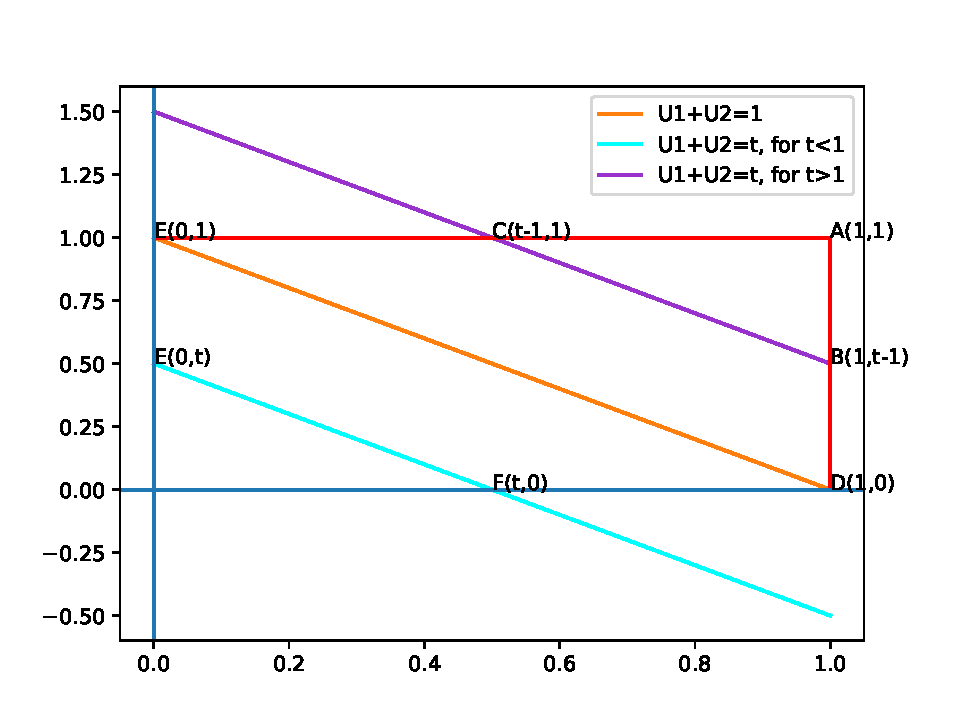
\includegraphics[width=\columnwidth]{figs/4/q4_2.pdf}
	 \caption{q4.2}
	\label{fig:q4_2}    
\end{figure}
Code for plot can be found at below link:
\begin{lstlisting}
	https://github.com/PradeepMundlik/AI1110/blob/master/Assignment_Soln/codes/4/q4_2.py
\end{lstlisting}
\begin{align}
	P(U_1+U_2 <t) &= \frac{\Delta EOF}{\Delta AEOD}\\
	 &= \frac{t^2}{2} \\
\end{align}
for $1 \leq t \leq 2$,
\begin{align}
	P(U_1+U_2 <t) &= \frac{\Delta ABC}{\Delta AEOD}\\
	 &= 1 - \frac{(2-t)^2}{2} 
\end{align}
\begin{align}
	 F_T(t) = 
	 \begin{cases}
		0 & t<0 \\
		\frac{t^2}{2} & 0 \leq t < 1 \\
		1 - \frac{(2-t)^2}{2} & 1 \leq t < 2 \\
		1 & t \geq 2
	 \end{cases}
\end{align}

\item Find the PDF of $T$. \\
\solution 
\begin{align}
	P_T(t) = \frac{d(F_T(t))}{dt} \\
	\therefore P_T(t) = 
	\begin{cases}
		0 & t < 0 \\
		t &  0 \leq t < 1 \\
		2-t & 1 \leq t < 2 \\
		0  & t \geq 2
	\end{cases}
\end{align}
\item Find the theoretical expressions for the PDF and CDF of $T$. \\
\solution 
\begin{align}
	F_T(t) =  
	 \begin{cases}
		0 & t<0 \\
		\frac{t^2}{2} & 0 \therefore \leq t < 1 \\
		1 - \frac{(2-t)^2}{2} & 1 \leq t < 2 \\
		1 & t \geq 2
	 \end{cases} \\
	 P_T(t) = 
	 \begin{cases}
		 0 & t < 0 \\
		 t &  0 \leq t < 1 \\
		 2-t & 1 \leq t < 2 \\
		 0  & t \geq 2
	 \end{cases}
\end{align}
\item Verify your results through a plot. \\
\solution 
Code files for plots can be found at:
\begin{lstlisting}
	https://github.com/PradeepMundlik/AI1110/blob/master/Assignment_Soln/codes/4/T_pdf.py
\end{lstlisting}
\begin{lstlisting}
	https://github.com/PradeepMundlik/AI1110/blob/master/Assignment_Soln/codes/4/T_cdf.py
\end{lstlisting}
PDF of T: fig \ref*{fig:T_pdf} \\
CDF of T: fig \ref*{fig:T_cdf}
\begin{figure}[h]
	\centering
	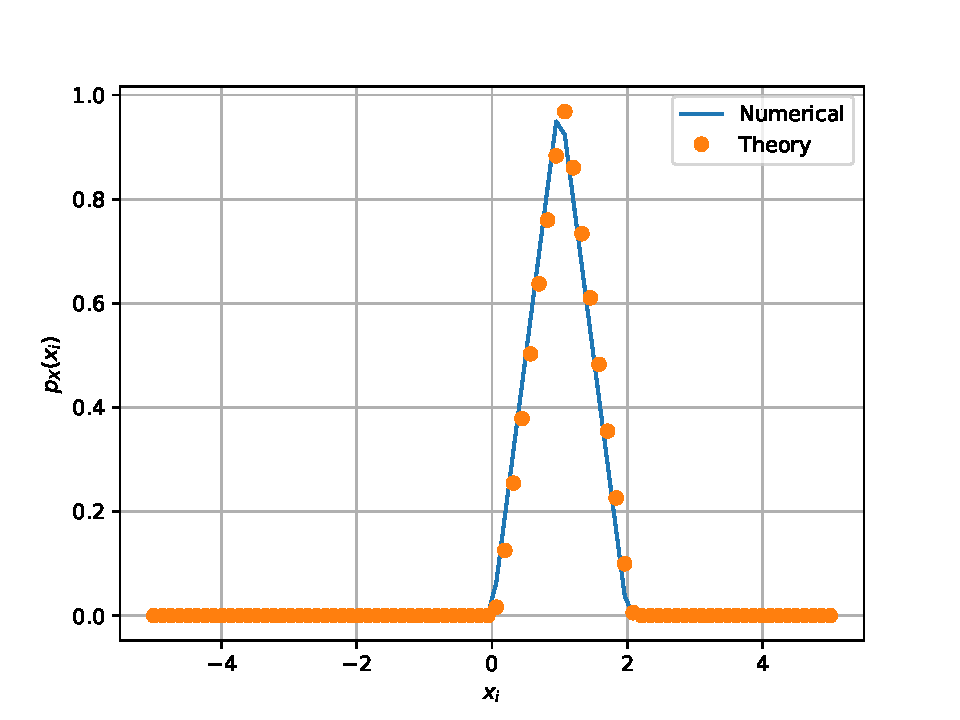
\includegraphics[width=\columnwidth]{figs/4/T_pdf.pdf}
	\caption{PDF of T}
	\label{fig:T_pdf}
\end{figure}
	\begin{figure}[h]
		\centering
		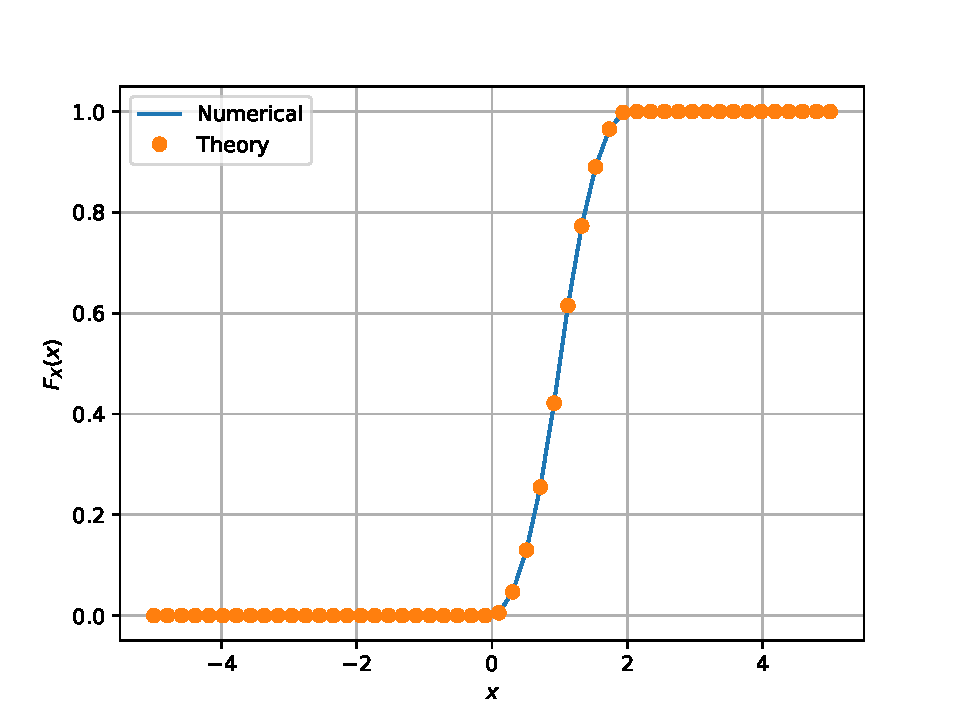
\includegraphics[width=\columnwidth]{figs/4/T_cdf.pdf}
		\caption{CDF of T}
		\label{fig:T_cdf}
\end{figure}
\end{enumerate}
% \section{Maximul Likelihood}
% \begin{enumerate}[label=\thesection.\arabic*
% ,ref=\thesection.\theenumi]
% \item Generate 
% \begin{equation}
% Y = AX+N,
% \end{equation}
% 		where $A = 5 \text{ dB}, X \i \cbrak{1,-1}$,  is Bernoulli and $N \sim \gauss{0}{1}$.
% 	\item Plot $Y$.
% 	\item Guess how to estimate $X$ from $Y$.
% \item
% \label{ml-ch4_sim}
% Find 
% \begin{equation}
% 	P_{e|0} = \pr{\hat{X} = -1|X=1}
% \end{equation}
% and 
% \begin{equation}
% 	P_{e|1} = \pr{\hat{X} = 1|X=-1}
% \end{equation}
% %
% \item Find $P_e$.

% %
% \item
% Verify by plotting  the theoretical $P_e$.  

% 		\end{enumerate}
% \section{Gaussian to Other}
% \begin{enumerate}[label=\thesection.\arabic*
% ,ref=\thesection.\theenumi]
% \item
% Let $X_1 \sim  \gauss{0}{1}$ and $X_2 \sim  \gauss{0}{1}$. Plot the CDF and PDF of
% %
% \begin{equation}
% V = X_1^2 + X_2^2
% \end{equation}
% %

% %
% %
% \item
% If
% %
% \begin{equation}
% F_{V}(x) = 
% \begin{cases}
% 1 - e^{-\alpha x} & x \geq 0 \\
% 0 & x < 0,
% \end{cases}
% \end{equation}
% %
% find $\alpha$.

% %
% \item
% \label{ch3_raleigh_sim}
% Plot the CDF and PDf of
% %
% \begin{equation}
% A = \sqrt{V}
% \end{equation}
% %


% \end{enumerate}

% \section{Conditional Probability}
% \begin{enumerate}[label=\thesection.\arabic*
% ,ref=\thesection.\theenumi]
% \item
% \item
% \label{ch4_sim}
% Plot 
% \begin{equation}
% P_e = \pr{\hat{X} = -1|X=1}
% \end{equation}
% %
% for 
% \begin{equation}
% Y = AX+N,
% \end{equation}
% where $A$ is Raleigh with $E\sbrak{A^2} = \gamma, N \sim \gauss{0}{1}, X \in \brak{-1,1}$ for $0 \le \gamma \le 10$ dB.

% %
% \item
% Assuming that $N$ is a constant, find an expression for $P_e$.  Call this $P_e(N)$

% %
% \item
% %
% \label{ch4_anal}
% For a function $g$,
% \begin{equation}
% E\sbrak{g(X)} = \int_{-\infty}^{\infty}g(x)p_{X}(x)\, dx
% \end{equation}
% %
% Find $P_e = E\sbrak{P_e(N)}$.

% %
% \item
% Plot $P_e$ in problems \ref{ch4_sim} and \ref{ch4_anal} on the same graph w.r.t $\gamma$.  Comment.

% 		\end{enumerate}
% \section{Two Dimensions}
% Let 
% \begin{equation}
% \mbf{y} = A\mbf{x} + \mbf{n},
% \end{equation}
% where 
% \begin{align}
% x &\in \brak{\mbf{s}_0,\mbf{s}_1}, 
% \mbf{s}_0 = 
% \begin{pmatrix}
% 1 
% \\
% 0
% \end{pmatrix},
% \mbf{s}_1 = 
% \begin{pmatrix}
% 0 
% \\
% 1
% \end{pmatrix}
% \\
% \mbf{n} &= 
% \begin{pmatrix}
% n_1
% \\
% n_2
% \end{pmatrix},
% n_1,n_2 \sim \gauss{0}{1}.
% \end{align}
% %
% \begin{enumerate}[label=\thesection.\arabic*
% ,ref=\thesection.\theenumi]

% %%
% \item
% \label{ch5_fsk}
% Plot 
% %
% \begin{equation}
% \mbf{y}|\mbf{s}_0 \text{ and } \mbf{y}|\mbf{s}_1
% \end{equation}
% %
% on the same graph using a scatter plot.

% %
% \item
% For the above problem, find a decision rule for detecting the symbols $\mbf{s}_0 $ and $\mbf{s}_1$.

% %
% \item
% Plot 
% \begin{equation} 
% P_e = \pr{\hat{\mbf{x}} = \mbf{s}_1|\mbf{x} = \mbf{s}_0}
% \end{equation}
% with respect to the SNR from 0 to 10 dB.

% %
% \item
% Obtain an expression for $P_e$. Verify this by comparing the theory and simulation plots on the same graph.

% %
% 		\end{enumerate}
\end{document}